\subsection{一次遅れと二次遅れ}

白線に沿って走る車輪型ロボットでは、カメラで検出した横ずれに応じて操舵角を変える。台車を目標位置へ戻すモータでは、位置のずれに応じて力や電圧を変える。サーモスタットや水槽の水位制御でも、測定値が目標から外れた分だけ加熱量や流入量を変える。いずれの例でも、目標値、測定値、その差、入力、出力を時間のグラフとして記録できる。

ON--OFF の切替だけで操作すると、誤差が小さくなった後も入力が急に変わるため、温度や水位は目標のまわりを往復しやすい。誤差に比例した入力へ置き換えても、比例係数が小さければ戻りが遅く、比例係数が大きければ行き過ぎや振動が現れる場合がある。したがって、制御器の式を書く前に、応答の速さ、目標値を越える量、振動の残り方、定常偏差を同じ尺度で評価できる形にする必要がある。

この目的に対して、すべての物理機構を最初から詳細に書く必要はない。出力が一つの蓄積量で決まり、入力を変えると指数関数的に新しい値へ近づく対象は、一次遅れによって応答の遅れと定常値を表せる。慣性やばねのように位置と速度の二つの量が関与し、目標値を越えたり振動したりする対象は、二次遅れによって減衰、収束、振動を表せる。

本節では、一次遅れと二次遅れを線形時不変系の最小の時間応答モデルとして定式化する。一次遅れでは時定数と静的ゲイン、二次遅れでは減衰比と固有角周波数を導入し、ステップ入力に対して応答速度、オーバーシュート、整定、定常偏差がどのように式とグラフに現れるかを確認する。

\begin{definition}[一次遅れ]
入力 $u(t)$ と出力 $y(t)$ が
\begin{equation}
  \tau\dot{y}(t)+y(t)=K u(t),\qquad \tau>0
  \label{eq:first-order}
\end{equation}
を満たすとき、これを一次遅れ系という。$\tau$ を時定数、$K$ を静的ゲインという。
\end{definition}

ステップ入力 $u(t)=u_0$ を加えたときの応答を導く。\weq{first-order} を
\begin{equation}
  \dot{y}(t)= -\frac{1}{\tau}y(t)+\frac{K}{\tau}u_0
\end{equation}
と書く。定常値 $y_\infty$ は $\dot{y}=0$ とおいて求める。
\begin{align}
  0&=-\frac{1}{\tau}y_\infty+\frac{K}{\tau}u_0,\\
  y_\infty&=K u_0.
\end{align}
そこで定常値からのずれ $z(t)=y(t)-y_\infty$ を考える。$y=z+y_\infty$、$\dot{y}=\dot{z}$ だから
\begin{align}
  \dot{z}
  &=-\frac{1}{\tau}(z+y_\infty)+\frac{K}{\tau}u_0\\
  &=-\frac{1}{\tau}z-\frac{1}{\tau}Ku_0+\frac{K}{\tau}u_0\\
  &=-\frac{1}{\tau}z.
\end{align}
一次の同次線形微分方程式の解より
\begin{equation}
  z(t)=z(0)e^{-t/\tau}
\end{equation}
である。$z(0)=y(0)-Ku_0$ なので
\begin{equation}
  y(t)=Ku_0+\{y(0)-Ku_0\}e^{-t/\tau}
  \label{eq:first-order-step}
\end{equation}
を得る。

時定数 $\tau$ は、偏差が初期偏差の $e^{-1}\simeq0.368$ 倍になる時刻である。この値は、\weq{first-order-step} に $t=\tau$ を代入して得られる。

\begin{figure}[tb]
\centering
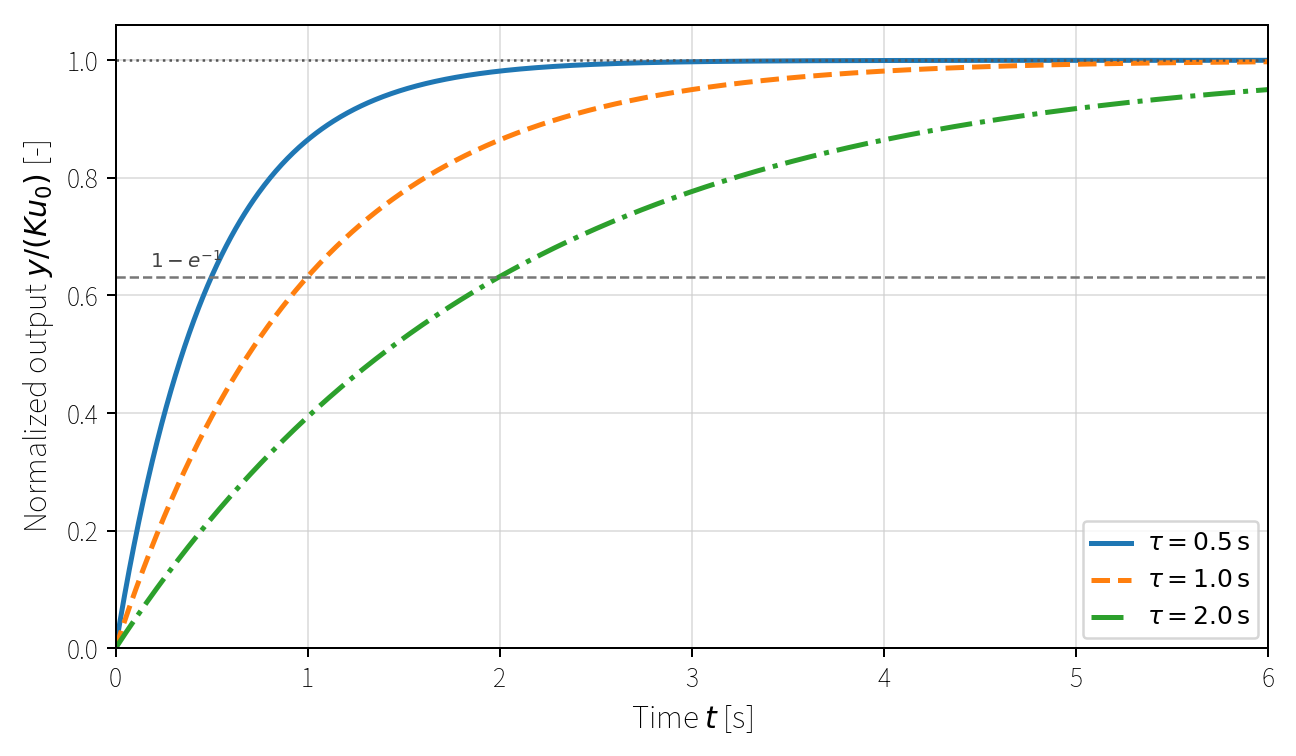
\includegraphics[width=\linewidth,bb=0 0 1296 756]{figures/time_response_first_order.png}
\caption{正規化した一次遅れ応答。$y/(Ku_0)=1-e^{-t/\tau}$ において時定数 $\tau$ だけを変えており、各曲線は $t=\tau$ で $1-e^{-1}$ に達する。}
\label{fig:first-order-time-response}
\end{figure}

\begin{figure}[tb]
\centering
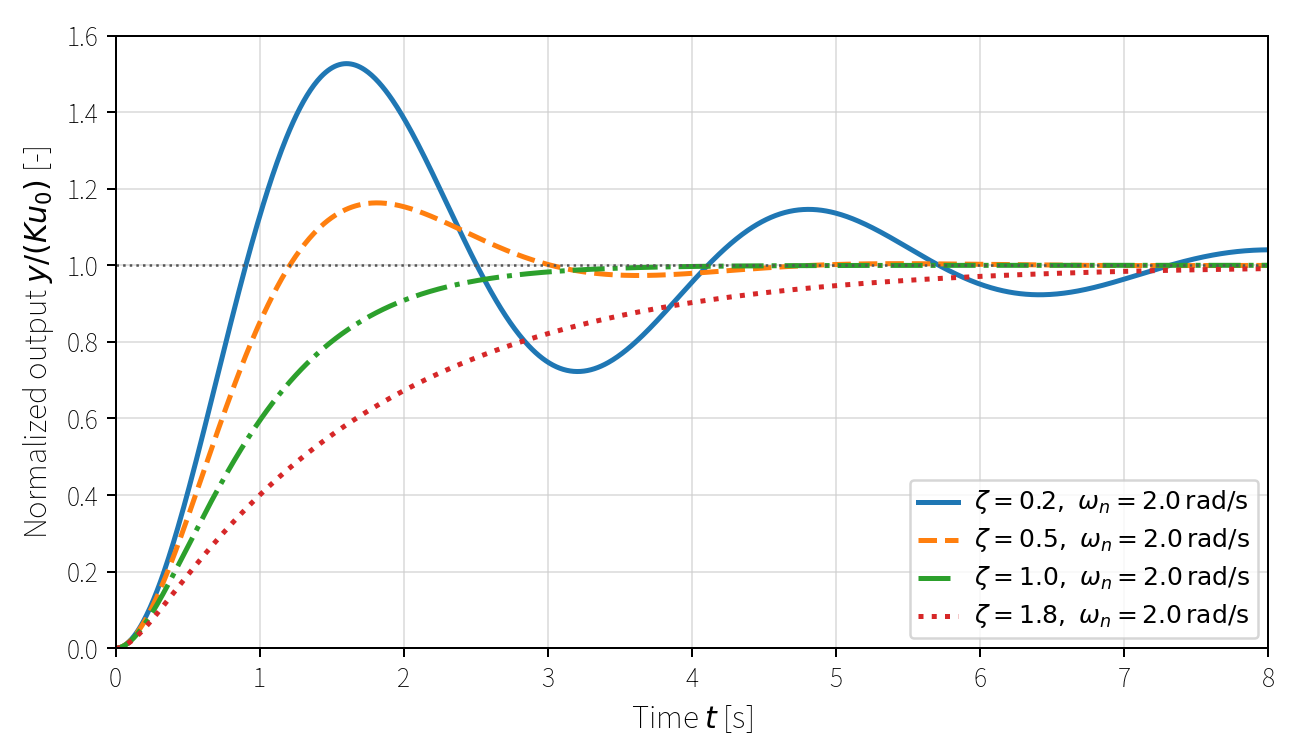
\includegraphics[width=\linewidth,bb=0 0 1296 756]{figures/time_response_second_order.png}
\caption{$\omega_n=2\,\mathrm{rad/s}$ を固定し、減衰比 $\zeta$ を変えた標準二次系の単位ステップ応答。減衰比により振動、オーバーシュート、整定の速さが変わる。}
\label{fig:time-response-examples}
\end{figure}

図\ref{fig:first-order-time-response} は、同じ静的ゲイン $K$ と同じステップ入力 $u_0$ に対して、時定数だけを変えた応答を正規化して示している。$\tau$ が小さいほど極 $-1/\tau$ は複素平面の左側へ移り、指数項 $e^{-t/\tau}$ が速く消えるため、定常値への接近も速くなる。一方、最終値 $Ku_0$ は時定数ではなく静的ゲインで決まる。図\ref{fig:time-response-examples} では、二次遅れ系の固有角周波数を固定し、減衰比 $\zeta$ だけを変えている。$\zeta<1$ では複素共役極が現れて振動とオーバーシュートが生じ、$\zeta=1$ は振動しない応答と振動応答の境界になり、$\zeta>1$ では二つの実極のうち遅い極が整定速度を支配する。

\begin{definition}[二次遅れの標準形]
出力 $y$ が
\begin{equation}
  \ddot{y}+2\zeta\omega_n\dot{y}+\omega_n^2 y=K\omega_n^2 u
  \label{eq:second-order}
\end{equation}
を満たすとき、これを二次遅れ系の標準形という。$\omega_n$ を固有角周波数、$\zeta$ を減衰比という。
\end{definition}

以後、この標準形では $\omega_n>0$、$\zeta\ge0$ とする。$\omega_n$ の単位は $\mathrm{rad/s}$ であり、$\zeta$ は無次元である。入力を一定値 $u(t)=u_0$ に保つと、定常値は $\dot{y}=\ddot{y}=0$ から
\begin{equation}
  y_\infty=K u_0
\end{equation}
である。偏差
\begin{equation}
  x(t)=y(t)-y_\infty
\end{equation}
を置くと、$u_0$ は相殺されて
\begin{equation}
  \ddot{x}+2\zeta\omega_n\dot{x}+\omega_n^2x=0
  \label{eq:second-order-deviation}
\end{equation}
となる。したがって二次系の形は、定常値そのものではなく、定常値からの偏差がどのように消えるかで決まる。入力を 0 とした自然応答は $u_0=0$ の特別な場合である。

\subsubsection{二次標準形の特性根}

\weq{second-order-deviation} に指数関数形 $x(t)=e^{st}$ を代入する。$e^{st}\ne0$ なので
\begin{equation}
  s^2+2\zeta\omega_n s+\omega_n^2=0
\end{equation}
を得る。これを二次系の特性方程式という。二次方程式の解の公式より
\begin{align}
  s&=\frac{-2\zeta\omega_n\pm
  \sqrt{(2\zeta\omega_n)^2-4\omega_n^2}}{2}\\
  &=-\zeta\omega_n\pm\omega_n\sqrt{\zeta^2-1}.
  \label{eq:second-order-characteristic-roots}
\end{align}
根の形は判別式、すなわち $\zeta^2-1$ の符号で三つに分かれる。この分類が、不足減衰、臨界減衰、過減衰である。

\subsubsection{不足減衰の応答}
$0<\zeta<1$ なら $\zeta^2-1<0$ なので、$\sqrt{\zeta^2-1}=j\sqrt{1-\zeta^2}$ と書ける。ここで
\begin{equation}
  \sigma=\zeta\omega_n,\qquad
  \omega_d=\omega_n\sqrt{1-\zeta^2}
\end{equation}
とおく。$\sigma$ は減衰係数、$\omega_d$ は減衰固有角周波数である。二つの極は
\begin{equation}
  s_{1,2}=-\sigma\pm j\omega_d
  \label{eq:second-order-poles}
\end{equation}
である。偏差応答は実関数として
\begin{equation}
  x(t)=e^{-\sigma t}
  \left(A\cos\omega_d t+B\sin\omega_d t\right)
  \label{eq:second-order-underdamped-free}
\end{equation}
と書ける。初期偏差を $x(0)=x_0$、初期速度を $\dot{x}(0)=v_0$ とすると
\begin{align}
  x(0)&=A=x_0,\\
  \dot{x}(0)&=-\sigma A+B\omega_d=v_0
\end{align}
だから
\begin{equation}
  A=x_0,\qquad
  B=\frac{v_0+\sigma x_0}{\omega_d}
  \label{eq:second-order-underdamped-constants}
\end{equation}
である。したがって $y(t)=K u_0+x(t)$ である。

初期静止 $y(0)=0$、$\dot{y}(0)=0$ から一定入力 $u(t)=u_0$ を加えるステップ応答では、$x_0=-K u_0$、$v_0=0$ である。これを \weq{second-order-underdamped-free} に代入して
\begin{equation}
  y(t)=K u_0\left[
    1-e^{-\sigma t}\left\{
      \cos\omega_d t+\frac{\sigma}{\omega_d}\sin\omega_d t
    \right\}
  \right]
  \label{eq:second-order-underdamped-step-general}
\end{equation}
を得る。不足減衰では、極の実部 $-\sigma=-\zeta\omega_n$ が包絡線 $e^{-\sigma t}$ の消え方を決め、虚部 $\omega_d$ が振動の角周波数を決める。$\zeta$ が小さいほど振動は強く残り、$\zeta$ が 1 に近づくほど $\omega_d$ は小さくなる。$\zeta=0$ は減衰を持たない境界であり、極は $\pm j\omega_n$ となって振幅が減衰しない。

\subsubsection{臨界減衰の応答}
$\zeta=1$ なら特性方程式は
\begin{equation}
  s^2+2\omega_n s+\omega_n^2=(s+\omega_n)^2=0
\end{equation}
となり、極は
\begin{equation}
  s=-\omega_n
\end{equation}
の重根である。重根では、指数関数 $e^{-\omega_n t}$ だけでは二階微分方程式の二つの初期条件を満たせないため、もう一つの独立解として $t e^{-\omega_n t}$ が現れる。偏差応答は
\begin{equation}
  x(t)=(A+Bt)e^{-\omega_n t}
  \label{eq:second-order-critical-free}
\end{equation}
である。初期値を代入すると
\begin{align}
  x(0)&=A=x_0,\\
  \dot{x}(0)&=B-\omega_n A=v_0
\end{align}
だから
\begin{equation}
  A=x_0,\qquad
  B=v_0+\omega_n x_0
  \label{eq:second-order-critical-constants}
\end{equation}
である。

初期静止から一定入力 $u_0$ を加えると、$x_0=-K u_0$、$v_0=0$ なので
\begin{equation}
  y(t)=K u_0\left\{1-(1+\omega_n t)e^{-\omega_n t}\right\}
  \label{eq:second-order-critical-step}
\end{equation}
となる。臨界減衰は、振動を伴わない応答と振動を伴う応答の境界である。初期静止からの正のステップ応答では、出力は振動せず単調に定常値へ近づく。同じ $\omega_n$ のもとで、$\zeta<1$ では複素共役極により振動が現れ、$\zeta>1$ では二つの実極に分かれて遅い実指数モードが支配的になる。

\subsubsection{過減衰の応答}
$\zeta>1$ なら二つの極は相異なる負の実数である。便宜上
\begin{align}
  p_1&=-\omega_n\left(\zeta-\sqrt{\zeta^2-1}\right),\\
  p_2&=-\omega_n\left(\zeta+\sqrt{\zeta^2-1}\right)
\end{align}
とおくと、$p_2<p_1<0$ である。偏差応答は
\begin{equation}
  x(t)=A e^{p_1t}+B e^{p_2t}
  \label{eq:second-order-overdamped-free}
\end{equation}
であり、初期条件から
\begin{align}
  A+B&=x_0,\\
  p_1A+p_2B&=v_0
\end{align}
を満たす。これを解くと
\begin{equation}
  A=\frac{v_0-p_2x_0}{p_1-p_2},\qquad
  B=\frac{p_1x_0-v_0}{p_1-p_2}
  \label{eq:second-order-overdamped-constants}
\end{equation}
である。

初期静止から一定入力 $u_0$ を加えるステップ応答では
\begin{equation}
  y(t)=K u_0\left[
    1+\frac{p_2}{p_1-p_2}e^{p_1t}
      -\frac{p_1}{p_1-p_2}e^{p_2t}
  \right]
  \label{eq:second-order-overdamped-step}
\end{equation}
となる。二つの指数はいずれも減衰するが、長時間では絶対値の小さい極 $p_1$ に対応する $e^{p_1t}$ が残る。$\zeta$ を非常に大きくすると $p_2$ は大きな負値へ移る一方で、$p_1$ は原点に近づくため、減衰を増やせば常に応答が速くなるわけではない。

図\ref{fig:time-response-examples} は、この三つの減衰分類を同じ時間軸で比較している。$\zeta=0.2$ の曲線は実部 $-\zeta\omega_n$ が小さいため包絡線の減衰が遅く、虚部に対応する振動が定常値を大きく超える。$\zeta=0.5$ では振動とオーバーシュートは残るが、包絡線は速く縮む。$\zeta=1$ は重根に対応し、初期静止からのステップ応答では定常値を越えずに近づく。$\zeta=1.8$ は過減衰であり、振動しないが遅い実極が原点に近いため、臨界減衰よりも整定が遅くなる。

\subsubsection{応答図による時定数と減衰比の検証}

図\ref{fig:first-order-time-response} では、一次遅れの正規化応答
$y/(Ku_0)=1-e^{-t/\tau}$ が、必ず $t=\tau$ で
$1-e^{-1}\simeq0.632$ に達する。したがって
$\tau=0.5\,\mathrm{s}$、$1.0\,\mathrm{s}$、$2.0\,\mathrm{s}$ の曲線は、それぞれ $0.5\,\mathrm{s}$、$1.0\,\mathrm{s}$、$2.0\,\mathrm{s}$ で同じ正規化高さを通る。対応する極は $-2.0\,\mathrm{s^{-1}}$、$-1.0\,\mathrm{s^{-1}}$、$-0.5\,\mathrm{s^{-1}}$ であり、極が左へ離れるほど指数項が速く消える。

図\ref{fig:time-response-examples} の二次応答も、極の位置で整理できる。$\omega_n=2\,\mathrm{rad/s}$ を固定すると、$\zeta=0.2$ では極の実部が $-0.4$ と小さく、振動の包絡線がゆっくり減るため、大きなオーバーシュートが残る。$\zeta=0.5$ では実部が $-1.0$ になり、振動は残るが減衰は速くなる。$\zeta=1.0$ では重根 $-2.0$ となり、初期静止からのステップ応答はオーバーシュートせずに定常値へ近づく。$\zeta=1.8$ では二つの実極がおよそ $-0.61$ と $-6.59$ に分かれ、長時間では原点に近い遅い極 $-0.61$ が支配する。そのため、減衰比を大きくすれば常に整定が速くなるわけではなく、過減衰では遅い実極が応答を引き伸ばす。

\subsubsection{ステップ応答の過渡仕様}

制御系の時間応答は、式全体だけでなく、グラフから算出できる少数の仕様値でも評価する。ここでは、時刻 $0$ で入力または目標値が一定値へ変わり、出力 $y(t)$ が有限な定常値へ収束する場合を考える。初期値を $y_0=y(0+)$、定常値を
\begin{equation}
  y_\infty=\lim_{t\to\infty}y(t)
\end{equation}
とし、応答の大きさを
\begin{equation}
  \Delta y=y_\infty-y_0
\end{equation}
で表す。以下の定義では $\Delta y>0$ の上向きステップを基準に書く。下向きステップでは、$y-y_0$ を $\Delta y$ で割った正規化応答で同じ定義を使う。

\begin{definition}[定常値と定常偏差]
出力が有限な極限を持つとき、その極限
\begin{equation}
  y_\infty=\lim_{t\to\infty}y(t)
\end{equation}
を定常値という。目標値または入力指令を $r(t)$ とし、$r_\infty=\lim_{t\to\infty}r(t)$ が存在するとき、
\begin{equation}
  e_\infty=\lim_{t\to\infty}\{r(t)-y(t)\}=r_\infty-y_\infty
  \label{eq:steady-state-error}
\end{equation}
を定常偏差という。単位ステップ目標に対して $y_\infty=1$ なら $e_\infty=0$ であり、出力が $0.98$ に収束するなら $e_\infty=0.02$ である。
\end{definition}

\begin{definition}[立上り時間、ピーク時刻、最大オーバーシュート、整定時間]
正規化応答を
\begin{equation}
  \eta(t)=\frac{y(t)-y_0}{\Delta y}
\end{equation}
とする。$\eta=0$ が初期値、$\eta=1$ が定常値に対応する。
\begin{itemize}
  \item 立上り時間は、応答が所定の下側割合から上側割合へ到達するまでの時間である。本書では測定値として、特に断らない限り $10\%$ から $90\%$ までの時間
  \begin{equation}
    t_r^{10-90}=t_{0.9}-t_{0.1},
    \qquad \eta(t_{0.1})=0.1,\quad \eta(t_{0.9})=0.9
  \end{equation}
  を用いる。標準二次系の公式では、初めて定常値に到達する $0$--$100\%$ 立上り時間もよく用いられる。
  \item ピーク時刻 $t_p$ は、ステップ後の最初の局所最大値に到達する時刻である。
  \item 最大オーバーシュート $M_p$ は、最大値 $y_{\max}$ が定常値をどれだけ超えたかを、変化量で割った値
  \begin{equation}
    M_p=\frac{y_{\max}-y_\infty}{\abs{\Delta y}}
  \end{equation}
  である。百分率では $100M_p\,\%$ と書く。
  \item $\varepsilon$ 整定時間 $t_s^{(\varepsilon)}$ は、時刻 $t_s^{(\varepsilon)}$ 以後に応答が定常値まわりの帯域
  \begin{equation}
    \abs{y(t)-y_\infty}\le \varepsilon\abs{\Delta y}
    \qquad (t\ge t_s^{(\varepsilon)})
  \end{equation}
  に入り続ける最初の時刻である。代表的には $\varepsilon=0.02$ の $2\%$ 整定時間と、$\varepsilon=0.05$ の $5\%$ 整定時間を使う。
\end{itemize}
\end{definition}

ステップ応答のグラフ上でこれらを求めるときは、まず最終的に落ち着く水平線 $y=y_\infty$ を決める。次に、初期値 $y_0$ から定常値 $y_\infty$ までの差 $\Delta y$ を基準に、$10\%$ 線 $y_0+0.1\Delta y$、$90\%$ 線 $y_0+0.9\Delta y$、必要なら $100\%$ 線 $y_\infty$ を引く。応答曲線が $10\%$ 線と $90\%$ 線を最初に横切る時刻の差が $10$--$90\%$ 立上り時間である。最初の山の頂点の横座標がピーク時刻、縦座標が $y_{\max}$ であり、$y_{\max}-y_\infty$ を $\abs{\Delta y}$ で割れば最大オーバーシュートになる。整定時間は、$y_\infty\pm\varepsilon\abs{\Delta y}$ の二本の水平線でできる帯域を描き、その帯域へ最後に入ったあとの時刻として定める。単に一度帯域に入った時刻ではなく、その後に帯域を出ないことまで含める点が重要である。

\begin{formula}[不足減衰二次系の標準過渡仕様]
次の仮定を置く。
\begin{itemize}
  \item 系は零点を持たない標準二次系
  \begin{equation}
    G(s)=\frac{K\omega_n^2}
             {s^2+2\zeta\omega_n s+\omega_n^2}
  \end{equation}
  で近似できる。
  \item $0<\zeta<1$、$\omega_n>0$ である。
  \item 初期静止状態から大きさ $u_0$ のステップを加え、$K u_0>0$ とする。
  \item 他の極はこの複素共役極より十分速く減衰し、測定ノイズや飽和は過渡仕様の評価を支配しない。
\end{itemize}
このとき、$\omega_d=\omega_n\sqrt{1-\zeta^2}$、$\sigma=\zeta\omega_n$ とおけば、定常値は
\begin{equation}
  y_\infty=K u_0
\end{equation}
であり、正規化応答は
\begin{equation}
  \eta(t)=1-e^{-\sigma t}
  \left\{\cos\omega_d t+\frac{\zeta}{\sqrt{1-\zeta^2}}\sin\omega_d t\right\}.
  \label{eq:transient-normalized-step}
\end{equation}
標準的な仕様値は
\begin{align}
  t_r^{0-100}
  &=\frac{\pi-\arccos\zeta}{\omega_d},
  \label{eq:rise-time-first-crossing}\\
  t_p
  &=\frac{\pi}{\omega_d},
  \label{eq:peak-time}\\
  M_p
  &=\exp\left(-\frac{\pi\zeta}{\sqrt{1-\zeta^2}}\right),
  \label{eq:maximum-overshoot}\\
  t_s^{(0.02)}
  &\simeq \frac{4}{\zeta\omega_n},
  \qquad
  t_s^{(0.05)}
  \simeq \frac{3}{\zeta\omega_n}.
  \label{eq:settling-time-envelope}
\end{align}
\weq{rise-time-first-crossing} は初回定常値到達時刻、\weq{peak-time} と \weq{maximum-overshoot} は標準二次系では厳密な式である。一方、整定時間の式は、減衰包絡 $e^{-\zeta\omega_n t}$ が $2\%$ または $5\%$ 程度まで小さくなる時刻を使った近似である。
\end{formula}

\weq{transient-normalized-step} の中括弧は、次のように一つの正弦波へまとめられる。$\phi=\arccos\zeta$ とおくと、$\sin\phi=\sqrt{1-\zeta^2}$ であるから
\begin{align}
  \cos\omega_d t
  +\frac{\zeta}{\sqrt{1-\zeta^2}}\sin\omega_d t
  &=
  \frac{1}{\sqrt{1-\zeta^2}}
  \sin(\omega_d t+\phi).
\end{align}
応答が初めて $\eta(t)=1$ に達するには、この正弦項が初めて 0 になればよい。$t=0$ では角度が $\phi$ であり、次の零点は $\omega_d t+\phi=\pi$ だから
\begin{equation}
  t_r^{0-100}=\frac{\pi-\phi}{\omega_d}
  =\frac{\pi-\arccos\zeta}{\omega_d}
\end{equation}
である。

ピーク時刻は $\dot{\eta}(t)=0$ で求める。\weq{transient-normalized-step} を微分すると
\begin{align}
  \dot{\eta}(t)
  &=
  e^{-\sigma t}
  \left[
    \sigma\left\{\cos\omega_d t+
    \frac{\sigma}{\omega_d}\sin\omega_d t\right\}
    +\omega_d\sin\omega_d t-\sigma\cos\omega_d t
  \right]\\
  &=
  e^{-\sigma t}
  \left(\omega_d+\frac{\sigma^2}{\omega_d}\right)\sin\omega_d t.
\end{align}
したがって極値は $\sin\omega_d t=0$、すなわち $t=k\pi/\omega_d$ で生じる。最初の正の極値は
\begin{equation}
  t_p=\frac{\pi}{\omega_d}
\end{equation}
である。この時刻では $\cos\pi=-1$、$\sin\pi=0$ なので
\begin{equation}
  \eta(t_p)
  =1+e^{-\sigma\pi/\omega_d}.
\end{equation}
よって
\begin{equation}
  M_p=\eta(t_p)-1
  =
  \exp\left(-\frac{\sigma\pi}{\omega_d}\right)
  =
  \exp\left(-\frac{\pi\zeta}{\sqrt{1-\zeta^2}}\right)
\end{equation}
を得る。

整定時間は包絡線から近似する。正規化偏差 $\eta(t)-1$ は指数因子 $e^{-\sigma t}$ を持つため、主要な減衰速度は $\sigma=\zeta\omega_n$ である。$2\%$ 帯域なら
\begin{equation}
  e^{-\sigma t}\simeq0.02
\end{equation}
と置き、両辺の自然対数を取ると
\begin{equation}
  t\simeq\frac{-\ln0.02}{\sigma}
  =\frac{3.912\cdots}{\zeta\omega_n}
  \simeq \frac{4}{\zeta\omega_n}
\end{equation}
である。同様に $5\%$ 帯域では $-\ln0.05=2.996\cdots$ なので
\begin{equation}
  t_s^{(0.05)}\simeq\frac{3}{\zeta\omega_n}
\end{equation}
となる。

\begin{example}[標準二次系の過渡仕様]
単位ステップ入力に対する標準二次系
\begin{equation}
  G(s)=\frac{16}{s^2+4s+16}
\end{equation}
を考える。分母を
\begin{equation}
  s^2+2\zeta\omega_n s+\omega_n^2
\end{equation}
と比較すると、$\omega_n=4\,\mathrm{rad/s}$、$2\zeta\omega_n=4$ より $\zeta=0.5$ である。したがって
\begin{align}
  \omega_d&=4\sqrt{1-0.5^2}=3.464\cdots\,\mathrm{rad/s},\\
  y_\infty&=1
\end{align}
である。初回定常値到達時刻は
\begin{equation}
  t_r^{0-100}
  =
  \frac{\pi-\arccos(0.5)}{3.464\cdots}
  =
  0.605\cdots\,\mathrm{s}
\end{equation}
であり、ピーク時刻は
\begin{equation}
  t_p=\frac{\pi}{3.464\cdots}
  =0.907\cdots\,\mathrm{s}
\end{equation}
である。最大オーバーシュートは
\begin{equation}
  M_p
  =
  \exp\left(-\frac{\pi(0.5)}{\sqrt{1-0.5^2}}\right)
  =
  0.163\cdots
\end{equation}
だから、ピーク値はおよそ $1.163$、百分率表示では $16.3\%$ である。$2\%$ 整定時間と $5\%$ 整定時間の近似は
\begin{equation}
  t_s^{(0.02)}\simeq\frac{4}{0.5\cdot4}=2.0\,\mathrm{s},
  \qquad
  t_s^{(0.05)}\simeq\frac{3}{0.5\cdot4}=1.5\,\mathrm{s}
\end{equation}
となる。目標値も単位ステップであれば $r_\infty=1$ なので、定常偏差は $e_\infty=1-y_\infty=0$ である。
\end{example}

\begin{remark}[過渡仕様の適用範囲]
上の公式は、零点を持たない不足減衰二次標準形を前提にした仕様である。実際の伝達関数に零点があると、同じ極を持っていても立上り時間、ピーク値、初期の曲がり方は変わる。特に右半平面零点を持つ非最小位相系では、正のステップに対して出力が最初に負側へ動く逆応答が生じることがあり、単純な $0$--$100\%$ 立上り時間や最大オーバーシュートの解釈が曖昧になる。高次系を二次系で近似する場合も、残りの極が十分速く、零点の影響が小さいという支配極近似の条件を確認する必要がある。

測定データから仕様を求める場合には、ノイズ、量子化、サンプリング周期、外乱、入力飽和にも注意する。ノイズを含む信号は整定帯域を細かく出入りするため、瞬間値だけで整定時間を判定すると過大または過小に見積もる。実験では、平均化、低域通過フィルタ、一定時間だけ帯域内に留まるという判定窓を用い、フィルタによる遅れが立上り時間とピーク時刻を変えないかも併せて確認する。
\end{remark}
